\newpage
\section{\textbf{KẾT QUẢ THỰC NGHIỆM}}

\subsection{Trang chủ}
\begin{figure}[H]
	\centering
	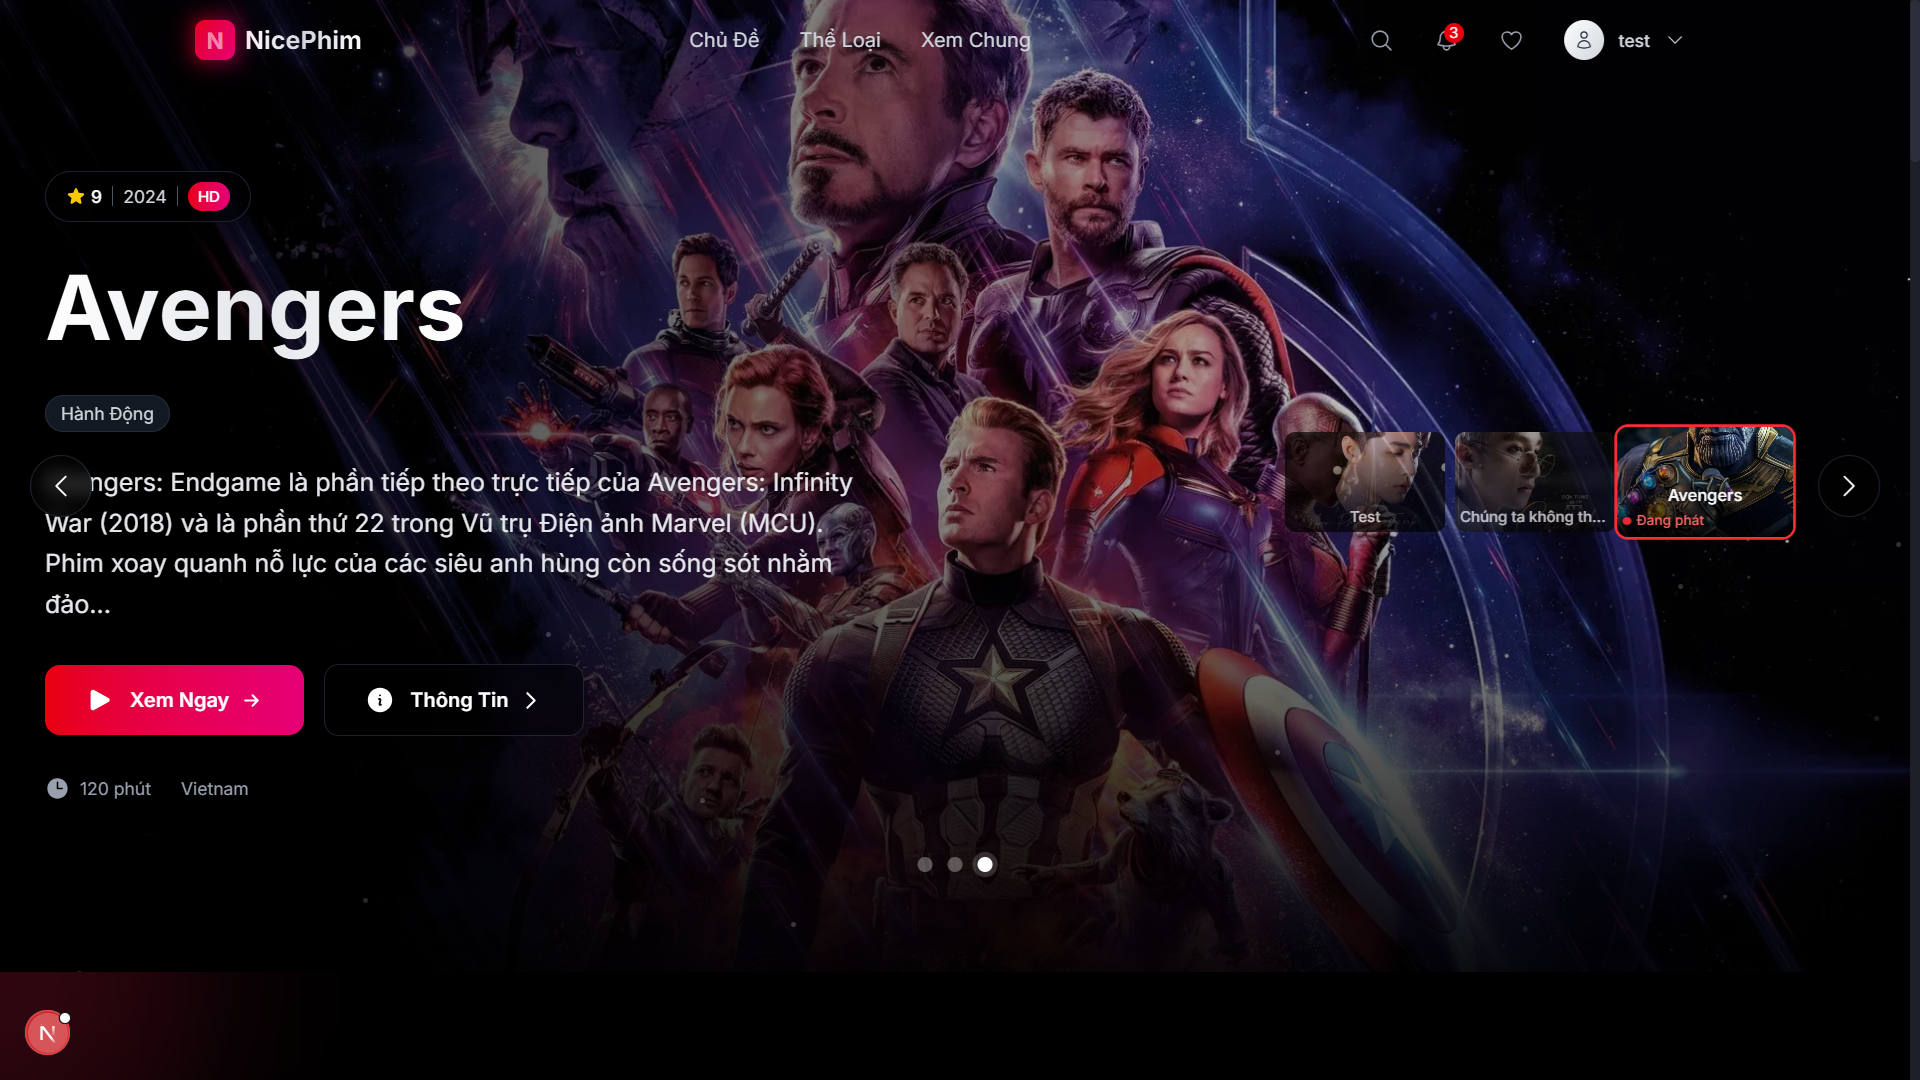
\includegraphics[width=0.9\textwidth]{image/demo/trangchu.png}
	\caption{Trang chủ}
\end{figure}

Trang chủ hiển thị giao diện chính của hệ thống với danh sách các bộ phim nổi bật, phim mới cập nhật và các danh mục phim được sắp xếp khoa học, giúp người dùng dễ dàng tìm kiếm và lựa chọn nội dung yêu thích.


\subsection{Chi tiết phim}
\begin{figure}[H]
	\centering
	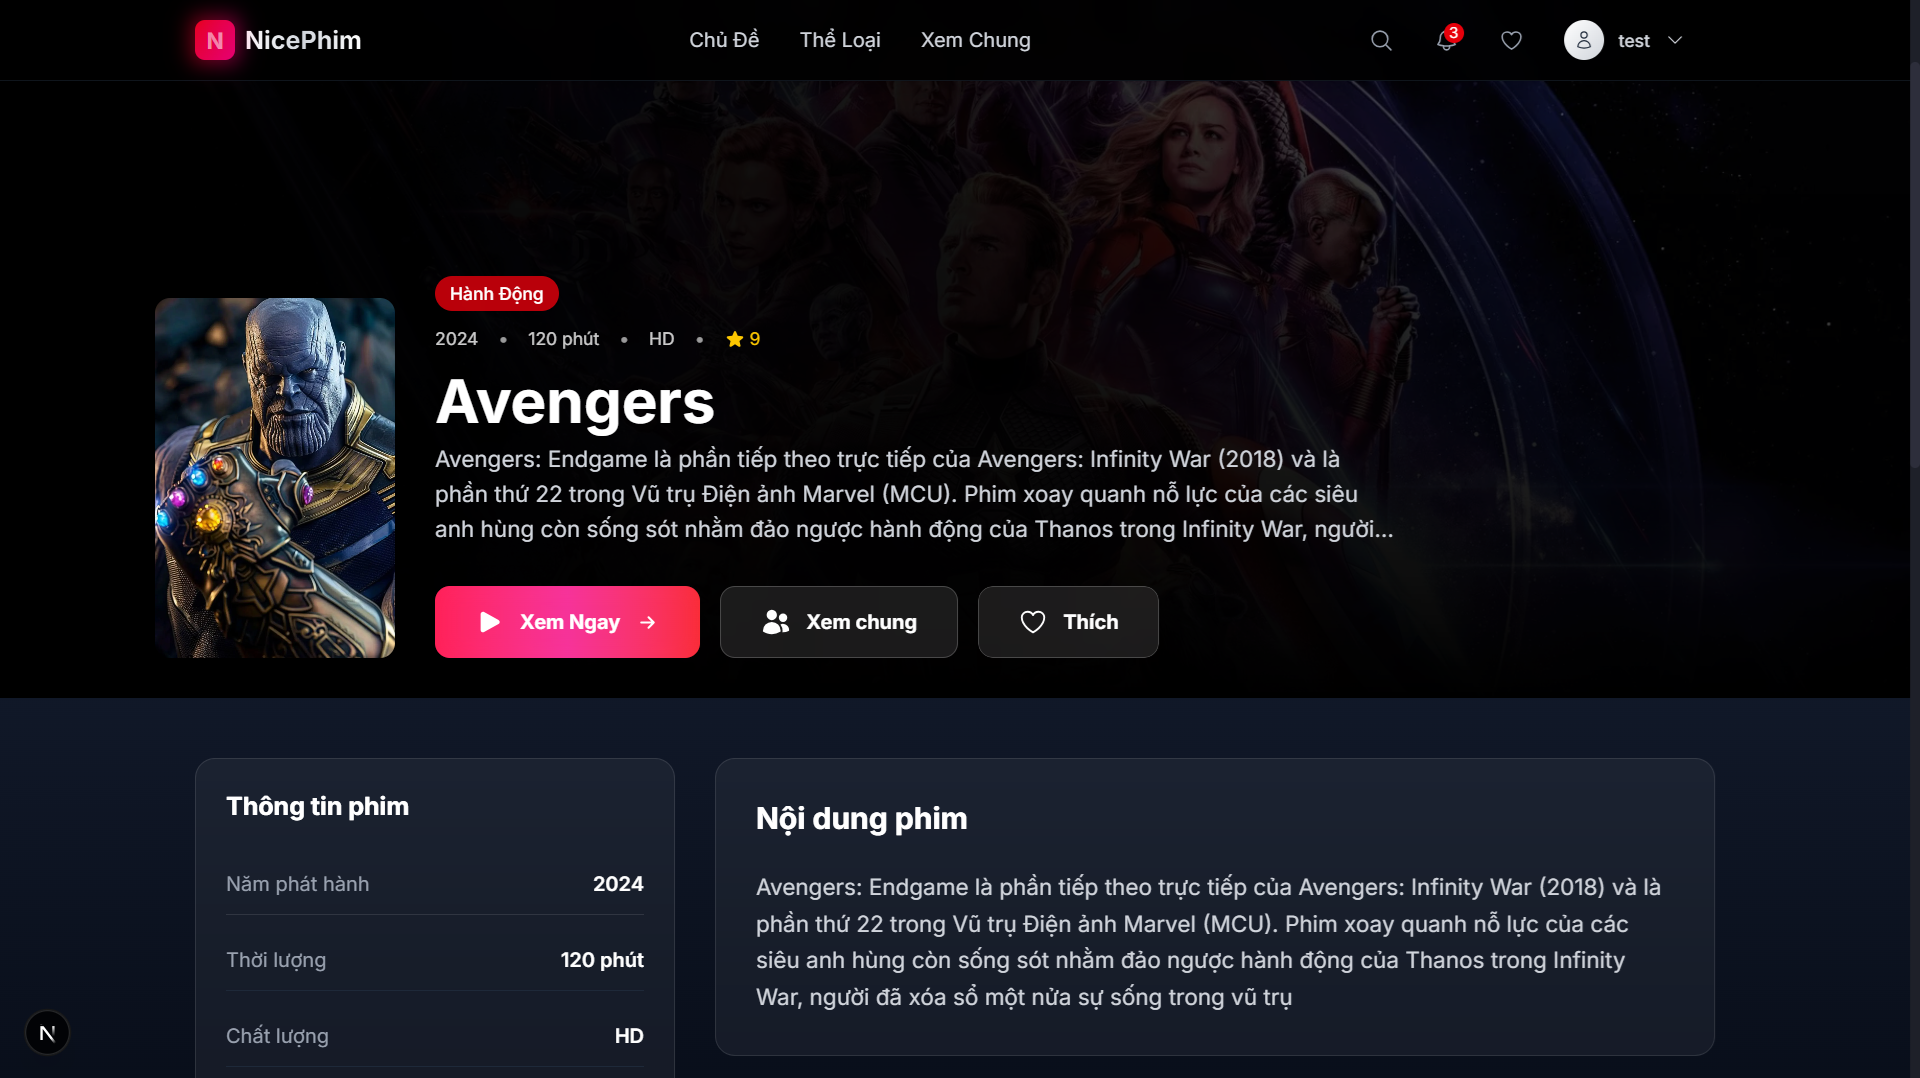
\includegraphics[width=0.9\textwidth]{image/demo/chitiet.png}
	\caption{Chi tiết phim}
\end{figure}

Trang chi tiết phim cung cấp thông tin đầy đủ về bộ phim bao gồm mô tả nội dung, thể loại, diễn viên, đạo diễn, thời lượng, đánh giá và các thông tin liên quan khác để người dùng có cái nhìn tổng quan trước khi xem.


\subsection{Xem phim cá nhân}
\begin{figure}[H]
	\centering
	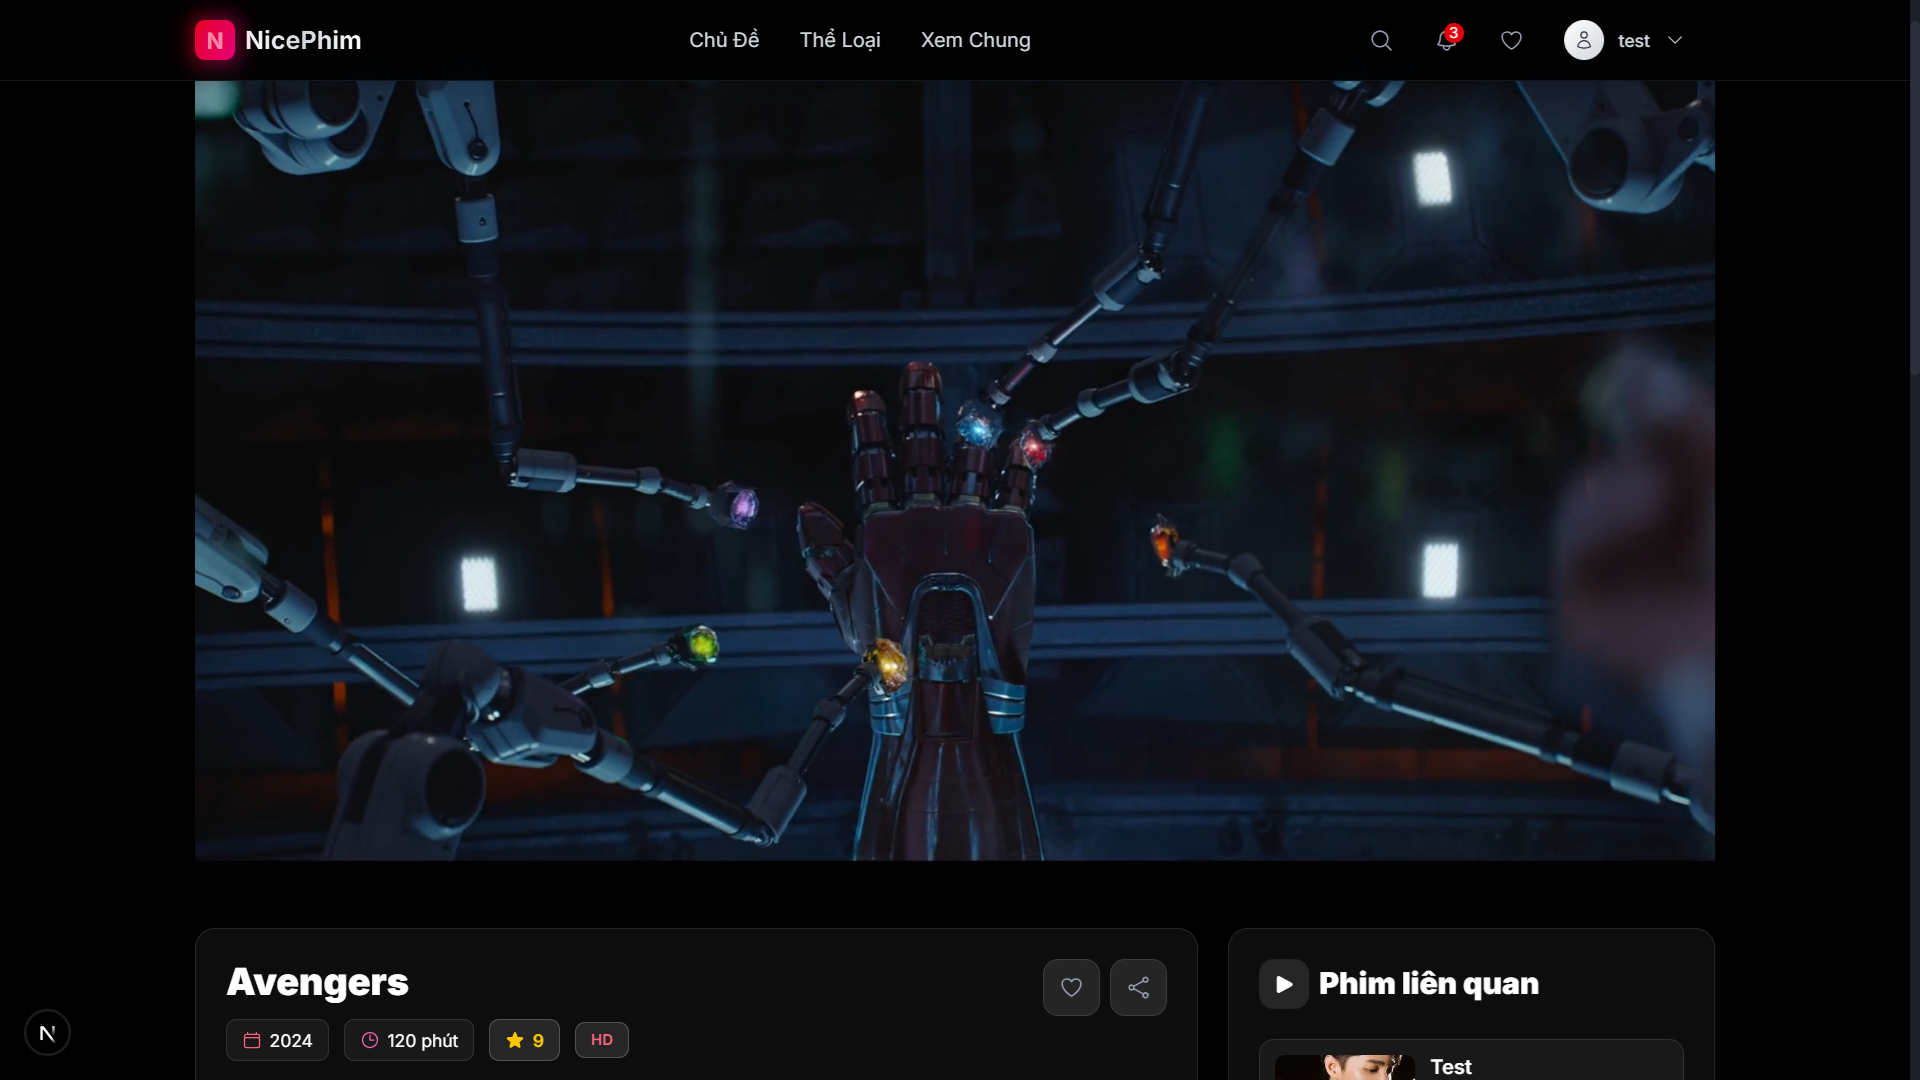
\includegraphics[width=0.9\textwidth]{image/demo/xemphim.png}
	\caption{Xem phim cá nhân}
\end{figure}

Giao diện xem phim cá nhân cung cấp trải nghiệm xem độc lập với trình phát video tích hợp đầy đủ chức năng điều khiển như play, pause, tua, điều chỉnh âm lượng và chế độ toàn màn hình.


\subsection{Tùy chọn chất lượng}
\begin{figure}[H]
	\centering
	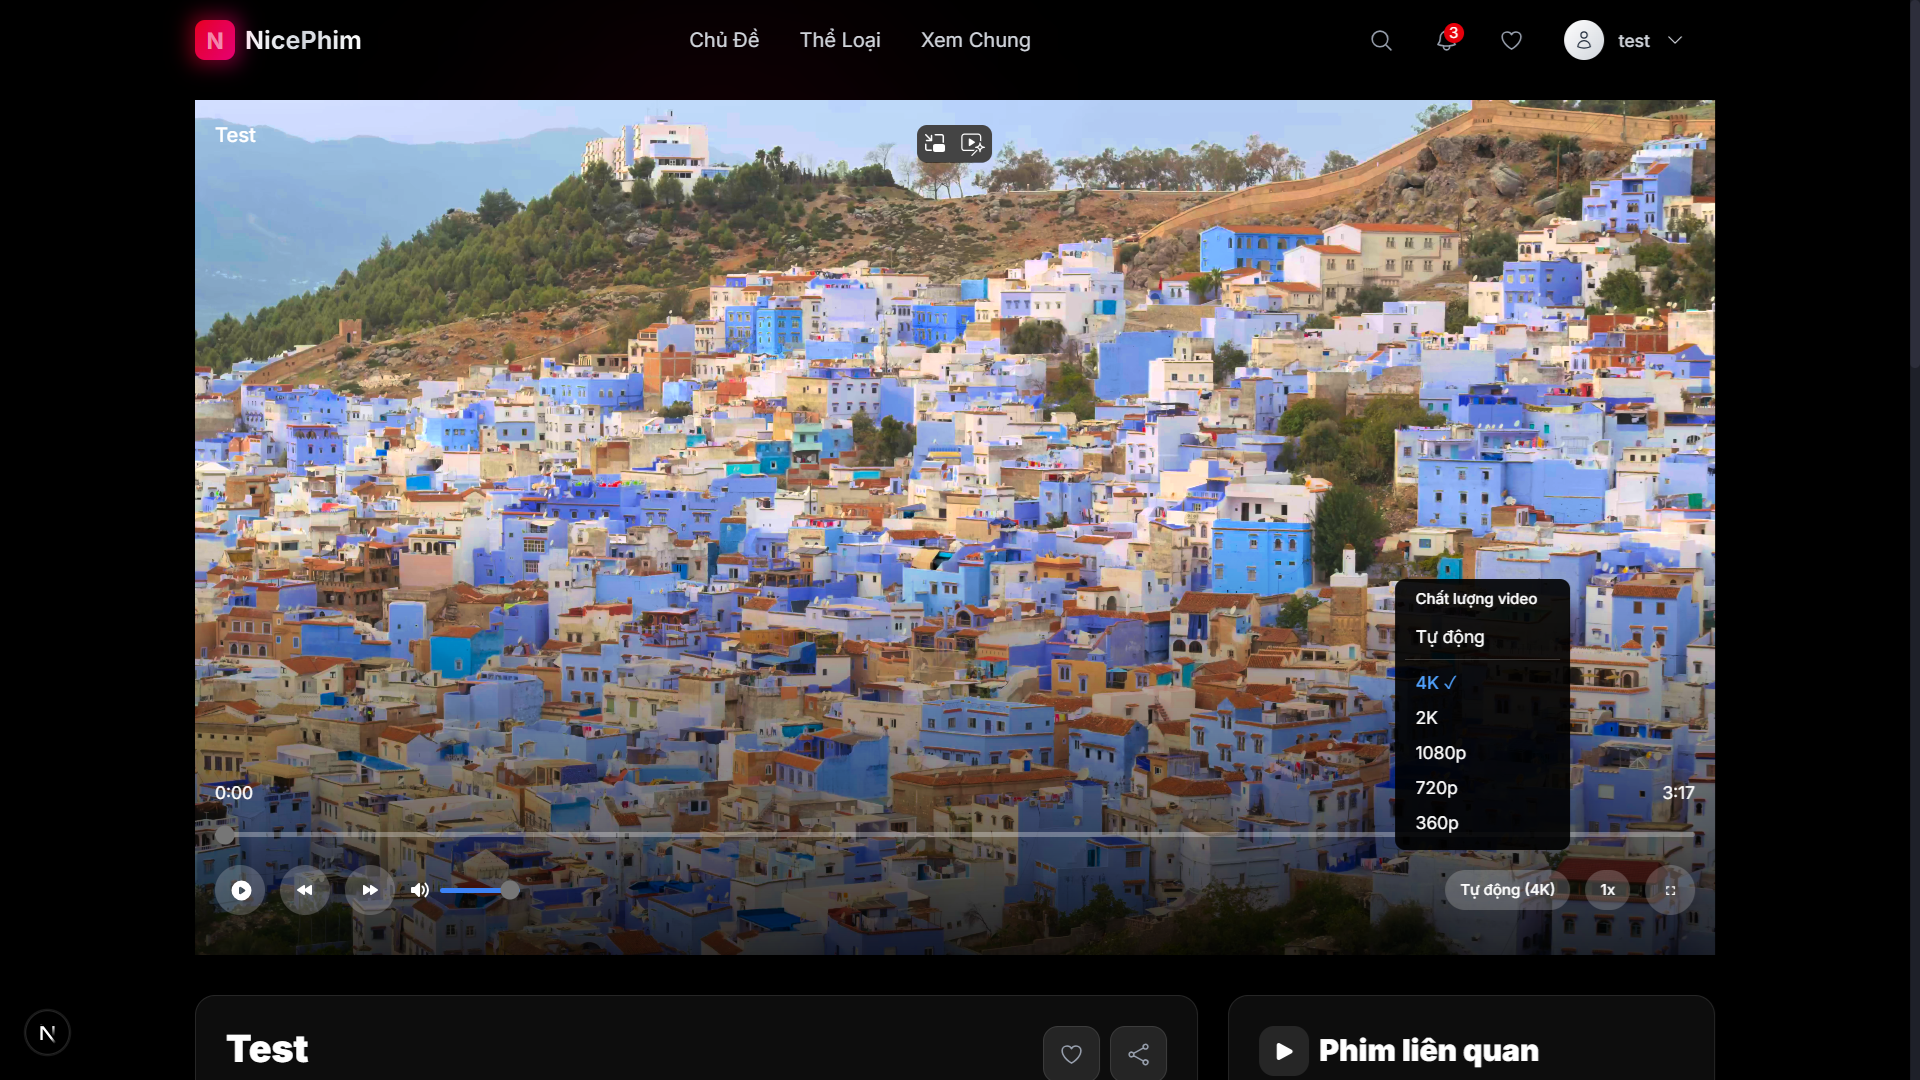
\includegraphics[width=0.9\textwidth]{image/demo/4K.png}
	\caption{Tùy chọn chất lượng}
\end{figure}

Hệ thống hỗ trợ người dùng lựa chọn chất lượng video phù hợp với băng thông mạng và thiết bị của mình, từ độ phân giải thấp đến cao như 720p, 1080p, 2K, 4K, đảm bảo trải nghiệm xem mượt mà.


\subsection{Chat thời gian thực}
\begin{figure}[H]
	\centering
	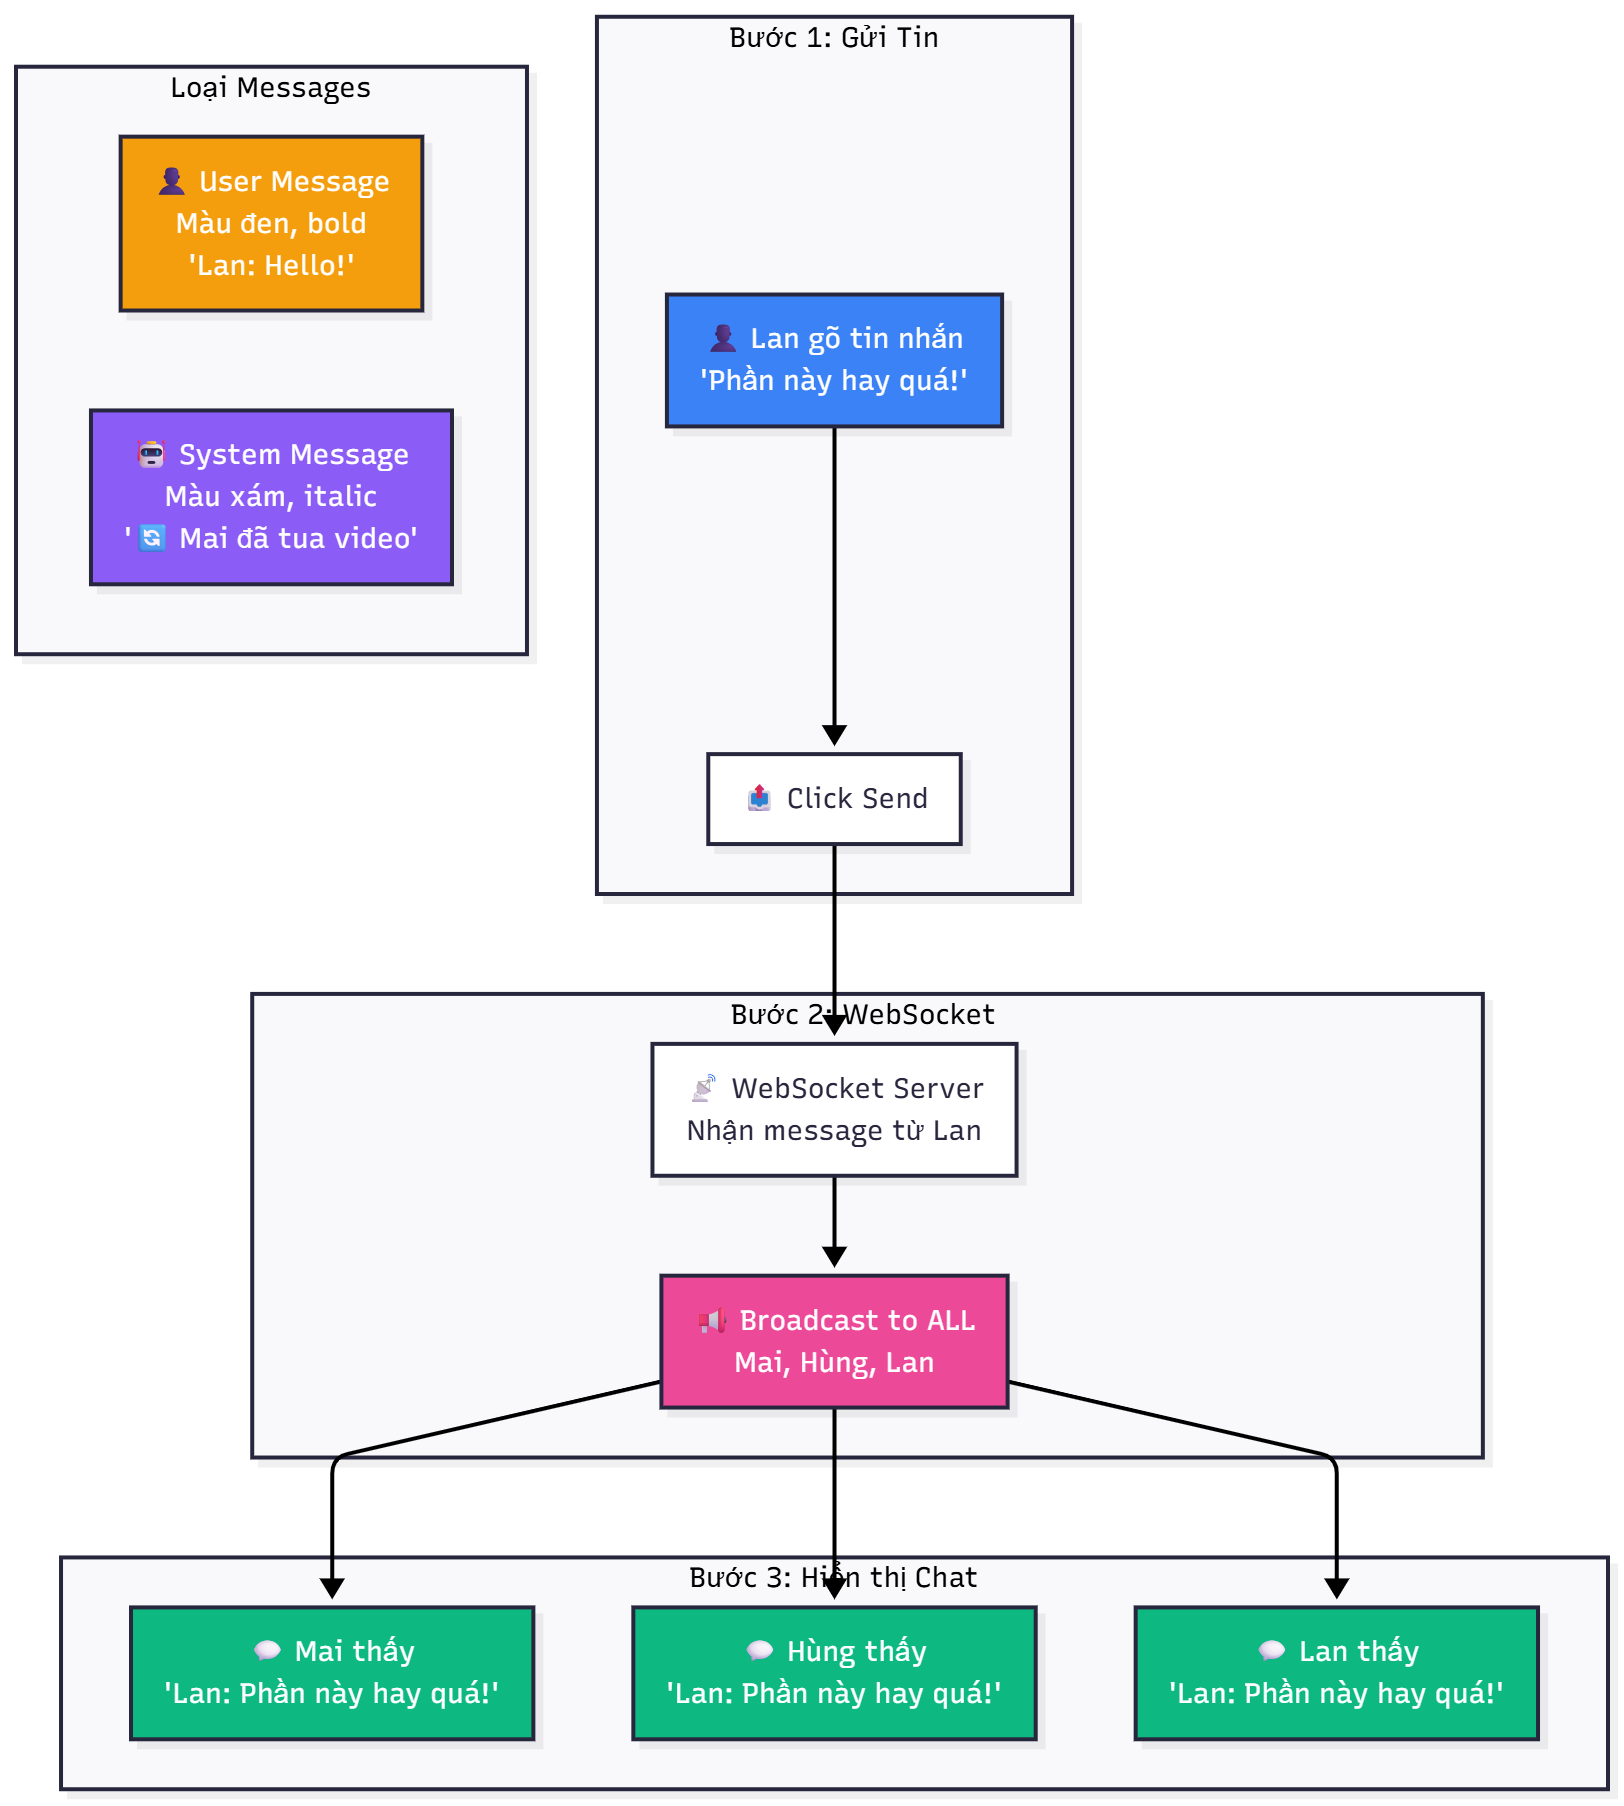
\includegraphics[width=0.9\textwidth]{image/demo/chat.png}
	\caption{Chat thời gian thực}
\end{figure}

Tính năng chat thời gian thực cho phép người dùng trao đổi, thảo luận về nội dung phim với những người xem khác hoặc liên hệ với bộ phận hỗ trợ, tạo sự tương tác và kết nối cộng đồng người dùng.

